\exercise

The following linked list L is expressed as a sequence of pairs $(i, succ(i))$
and item 4 is the head of the list: $L = \{ (1,6), (2,5), (3,0), (4,2), (5,1),
(6,3) \}$\footnote{We can assume the pair $(3, 0)$ represents the last element
of the list (with 0 as {\tt NULL} or ``no successor''), thus will be represented
from now on as $(3, 3)$, as in Prof. Ferragina's lecture notes.}. Show all the
steps needed to simulate the operation $succ(i) = succ(succ(i))$ of the Pointer
Jumping technique in the 2-levels model using a sequence of {\tt sort} and {\tt
scan}.

\solution

\autoref{fig:list1} shows the the initial state of the list $L$. To simulate the
Pointer Jumping technique in the 2-levels model we first have to store the list
as \emph{triples} $\langle i, succ(i), rank(i) \rangle$, initializing $rank(i) =
0$ if $succ(i) = i$ and $rank(i) = 1$ otherwise, as in \autoref{tab:list}. Then,
we store again the same list as \emph{quadruples} such as $\langle i, succ(i),
0, 0 \rangle$, wher the third and fourth component of the tuple are temporary
placeholders for the values of $rank(succ(i))$ and $succ(succ(i))$. Then proceed
updating the value of $rank(i)$ (in the triples) using a sequence of {\tt sort}
and {\tt scan} primitives, as follows:
%
\begin{align*}
  \text{\bf 1. }
  \begin{matrix}
    \langle 1, 6, 0, 0 \rangle \\
    \langle 2, 5, 0, 0 \rangle \\
    \langle 3, 3, 0, 0 \rangle \\
    \langle 4, 2, 0, 0 \rangle \\
    \langle 5, 1, 0, 0 \rangle \\
    \langle 6, 3, 0, 0 \rangle \\
  \end{matrix}
  \stackrel{\text{\tiny \tt sort}}{\longmapsto}
  \begin{matrix}
    \langle 5, 1, 0, 0 \rangle \\
    \langle 4, 2, 0, 0 \rangle \\
    \langle 3, 3, 0, 0 \rangle \\
    \langle 6, 3, 0, 0 \rangle \\
    \langle 2, 5, 0, 0 \rangle \\
    \langle 1, 6, 0, 0 \rangle \\
  \end{matrix}
  \stackrel{\text{\tiny \tt scan}}{\longmapsto}
  \begin{matrix}
    \langle 5, 1, 1, 6 \rangle \\
    \langle 4, 2, 1, 5 \rangle \\
    \langle 3, 3, 0, 3 \rangle \\
    \langle 6, 3, 0, 3 \rangle \\
    \langle 2, 5, 1, 1 \rangle \\
    \langle 1, 6, 1, 3 \rangle \\
  \end{matrix}
  \stackrel{\text{\tiny \tt sort}}{\longmapsto}
  \begin{matrix}
    \langle 1, 6, 1, 3 \rangle \\
    \langle 2, 5, 1, 1 \rangle \\
    \langle 3, 3, 0, 3 \rangle \\
    \langle 4, 2, 1, 5 \rangle \\
    \langle 5, 1, 1, 6 \rangle \\
    \langle 6, 3, 0, 3 \rangle \\
  \end{matrix}
  \stackrel{\text{\tiny \tt scan}}{\longmapsto}
  \begin{matrix}
    rank(1) + 1 = 2,\ succ(1) = 3 \\
    rank(2) + 1 = 2,\ succ(2) = 1 \\
    rank(3) + 0 = 0,\ succ(3) = 3 \\
    rank(4) + 1 = 2,\ succ(4) = 5 \\
    rank(5) + 1 = 2,\ succ(5) = 6 \\
    rank(6) + 0 = 1,\ succ(6) = 3 \\
  \end{matrix}
\end{align*}
%
\begin{align*}
  \text{\bf 2. }
  \begin{matrix}
    \langle 1, 3, 0, 0 \rangle \\
    \langle 2, 1, 0, 0 \rangle \\
    \langle 3, 3, 0, 0 \rangle \\
    \langle 4, 5, 0, 0 \rangle \\
    \langle 5, 6, 0, 0 \rangle \\
    \langle 6, 3, 0, 0 \rangle \\
  \end{matrix}
  \stackrel{\text{\tiny \tt sort}}{\longmapsto}
  \begin{matrix}
    \langle 2, 1, 0, 0 \rangle \\
    \langle 1, 3, 0, 0 \rangle \\
    \langle 3, 3, 0, 0 \rangle \\
    \langle 6, 3, 0, 0 \rangle \\
    \langle 4, 5, 0, 0 \rangle \\
    \langle 5, 6, 0, 0 \rangle \\
  \end{matrix}
  \stackrel{\text{\tiny \tt scan}}{\longmapsto}
  \begin{matrix}
    \langle 2, 1, 2, 3 \rangle \\
    \langle 1, 3, 0, 3 \rangle \\
    \langle 3, 3, 0, 3 \rangle \\
    \langle 6, 3, 0, 3 \rangle \\
    \langle 4, 5, 2, 6 \rangle \\
    \langle 5, 6, 1, 3 \rangle \\
  \end{matrix}
  \stackrel{\text{\tiny \tt sort}}{\longmapsto}
  \begin{matrix}
    \langle 1, 3, 0, 3 \rangle \\
    \langle 2, 1, 2, 3 \rangle \\
    \langle 3, 3, 0, 3 \rangle \\
    \langle 4, 5, 2, 6 \rangle \\
    \langle 5, 6, 1, 3 \rangle \\
    \langle 6, 3, 0, 3 \rangle \\
  \end{matrix}
  \stackrel{\text{\tiny \tt scan}}{\longmapsto}
  \begin{matrix}
    rank(1) + 0 = 2,\ succ(1) = 3 \\
    rank(2) + 2 = 4,\ succ(2) = 3 \\
    rank(3) + 0 = 0,\ succ(3) = 3 \\
    rank(4) + 2 = 4,\ succ(4) = 6 \\
    rank(5) + 1 = 3,\ succ(5) = 3 \\
    rank(6) + 0 = 1,\ succ(6) = 3 \\
  \end{matrix}
\end{align*}
%
\begin{align*}
  \text{\bf 3. }
  \begin{matrix}
    \langle 1, 3, 0, 0 \rangle \\
    \langle 2, 3, 0, 0 \rangle \\
    \langle 3, 3, 0, 0 \rangle \\
    \langle 4, 6, 0, 0 \rangle \\
    \langle 5, 3, 0, 0 \rangle \\
    \langle 6, 3, 0, 0 \rangle \\
  \end{matrix}
  \stackrel{\text{\tiny \tt sort}}{\longmapsto}
  \begin{matrix}
    \langle 1, 3, 0, 0 \rangle \\
    \langle 2, 3, 0, 0 \rangle \\
    \langle 3, 3, 0, 0 \rangle \\
    \langle 5, 3, 0, 0 \rangle \\
    \langle 6, 3, 0, 0 \rangle \\
    \langle 4, 6, 0, 0 \rangle \\
  \end{matrix}
  \stackrel{\text{\tiny \tt scan}}{\longmapsto}
  \begin{matrix}
    \langle 1, 3, 0, 3 \rangle \\
    \langle 2, 3, 0, 3 \rangle \\
    \langle 3, 3, 0, 3 \rangle \\
    \langle 5, 3, 0, 3 \rangle \\
    \langle 6, 3, 0, 3 \rangle \\
    \langle 4, 6, 1, 3 \rangle \\
  \end{matrix}
  \stackrel{\text{\tiny \tt sort}}{\longmapsto}
  \begin{matrix}
    \langle 1, 3, 0, 3 \rangle \\
    \langle 2, 3, 0, 3 \rangle \\
    \langle 3, 3, 0, 3 \rangle \\
    \langle 4, 6, 1, 3 \rangle \\
    \langle 5, 3, 0, 3 \rangle \\
    \langle 6, 3, 0, 3 \rangle \\
  \end{matrix}
  \stackrel{\text{\tiny \tt scan}}{\longmapsto}
  \begin{matrix}
    rank(1) + 0 = 2,\ succ(1) = 3 \\
    rank(2) + 0 = 4,\ succ(2) = 3 \\
    rank(3) + 0 = 0,\ succ(3) = 3 \\
    rank(4) + 1 = 5,\ succ(4) = 3 \\
    rank(5) + 0 = 3,\ succ(5) = 3 \\
    rank(6) + 0 = 1,\ succ(6) = 3 \\
  \end{matrix}
\end{align*}
%
\begin{figure} [t]
  \begin{subfigure}{\linewidth}
    \centering
    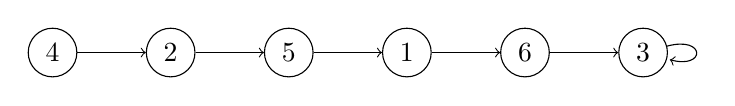
\begin{tikzpicture}[node distance=1.5cm, every node/.append style={draw,circle}]
      \node (a) {4};
      \node[right of=a] (b) {2};
      \node[right of=b] (c) {5};
      \node[right of=c] (d) {1};
      \node[right of=d] (e) {6};
      \node[right of=e] (f) {3};
      \draw[->] (a) -- (b);
      \draw[->] (b) -- (c);
      \draw[->] (c) -- (d);
      \draw[->] (d) -- (e);
      \draw[->] (e) -- (f);
      \path (f) edge[->, loop right] (f);
    \end{tikzpicture}
    \caption{Initial state.}
    \label{fig:list1}
  \end{subfigure} \vspace{1em} \\
  \begin{subfigure}{\linewidth}
    \centering
    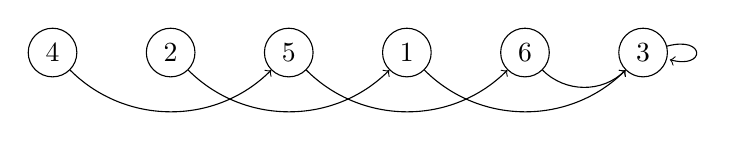
\begin{tikzpicture}[node distance=1.5cm, every node/.append style={draw,circle}]
      \node (a) {4};
      \node[right of=a] (b) {2};
      \node[right of=b] (c) {5};
      \node[right of=c] (d) {1};
      \node[right of=d] (e) {6};
      \node[right of=e] (f) {3};
      \path (a) edge[->, out=-45, in=-135] (c);
      \path (b) edge[->, out=-45, in=-135] (d);
      \path (c) edge[->, out=-45, in=-135] (e);
      \path (d) edge[->, out=-45, in=-135] (f);
      \path (e) edge[->, out=-45, in=-135] (f);
      \path (f) edge[->, loop right] (f);
    \end{tikzpicture}
    \caption{First step.}
    \label{fig:list2}
  \end{subfigure} \vspace{1em} \\
  \begin{subfigure}{\linewidth}
    \centering
    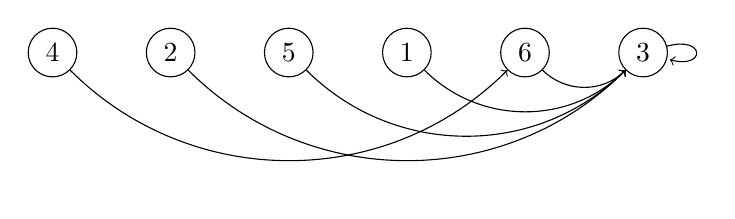
\begin{tikzpicture}[node distance=1.5cm, every node/.append style={draw,circle}]
      \node (a) {4};
      \node[right of=a] (b) {2};
      \node[right of=b] (c) {5};
      \node[right of=c] (d) {1};
      \node[right of=d] (e) {6};
      \node[right of=e] (f) {3};
      \path (a) edge[->, out=-45, in=-135] (e);
      \path (b) edge[->, out=-45, in=-135] (f);
      \path (c) edge[->, out=-45, in=-135] (f);
      \path (d) edge[->, out=-45, in=-135] (f);
      \path (e) edge[->, out=-45, in=-135] (f);
      \path (f) edge[->, loop right] (f);
    \end{tikzpicture}
    \caption{Second step.}
    \label{fig:list2}
  \end{subfigure} \vspace{1em} \\
  \begin{subfigure}{\linewidth}
    \centering
    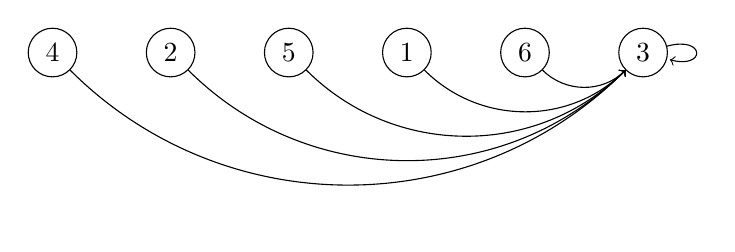
\begin{tikzpicture}[node distance=1.5cm, every node/.append style={draw,circle}]
      \node (a) {4};
      \node[right of=a] (b) {2};
      \node[right of=b] (c) {5};
      \node[right of=c] (d) {1};
      \node[right of=d] (e) {6};
      \node[right of=e] (f) {3};
      \path (a) edge[->, out=-45, in=-135] (f);
      \path (b) edge[->, out=-45, in=-135] (f);
      \path (c) edge[->, out=-45, in=-135] (f);
      \path (d) edge[->, out=-45, in=-135] (f);
      \path (e) edge[->, out=-45, in=-135] (f);
      \path (f) edge[->, loop right] (f);
    \end{tikzpicture}
    \caption{Third step.}
    \label{fig:list3}
  \end{subfigure}
  \caption{Graph representation of $L$.}
  \label{fig:list}
\end{figure}
%
\begin{table}[t]
  \centering
  \begin{tabular}{c|cccccc}
    $i$          & 1 & 2 & 3 & 4 & 5 & 6 \\ \hline\hline
    $succ(i)$    & 6 & 5 & 3 & 2 & 1 & 3 \\
    $rank(i)$    & 1 & 1 & 0 & 1 & 1 & 1 \\ \hline
    $succ'(i)$   & 3 & 1 & 3 & 5 & 6 & 3 \\
    $rank'(i)$   & 2 & 2 & 0 & 2 & 2 & 1 \\ \hline
    $succ''(i)$  & 3 & 3 & 3 & 6 & 3 & 3 \\
    $rank''(i)$  & 2 & 4 & 0 & 4 & 3 & 1 \\ \hline
    $succ'''(i)$ & 3 & 3 & 3 & 3 & 3 & 3 \\
    $rank'''(i)$ & 2 & 4 & 0 & 5 & 3 & 1 \\ \hline
  \end{tabular}
  \caption{Memory representation of $L$.}
  \label{tab:list}
\end{table}
